\documentclass[11pt, a4paper]{article}
\usepackage{pdfpages}
\usepackage{parallel}
\usepackage[T2A]{fontenc}
\usepackage{ucs}
\usepackage[utf8x]{inputenc}
\usepackage[polish,english,russian]{babel}
\usepackage{hyperref}
\usepackage{rotating}
\usepackage[inner=2cm,top=1.8cm,outer=2cm,bottom=2.3cm,nohead]{geometry}
\usepackage{listings}
\usepackage{graphicx}
\usepackage{wrapfig}
\usepackage{longtable}
\usepackage{indentfirst}
\usepackage{array}
\usepackage{tikzsymbols}
\usepackage{soul}
\usepackage[ruled,vlined]{algorithm2e}
%\counterwithout{figure}{section} 

\usepackage{url}
\makeatletter
\g@addto@macro{\UrlBreaks}{\UrlOrds}
\makeatother

\newcolumntype{P}[1]{>{\raggedright\arraybackslash}p{#1}}
\frenchspacing
\usepackage{fixltx2e} %text sub- and superscripts
\usepackage{icomma} % коскі ў матэматычным рэжыме
\PreloadUnicodePage{4}

\newcommand{\longpage}{\enlargethispage{\baselineskip}}
\newcommand{\shortpage}{\enlargethispage{-\baselineskip}}

\def\switchlang#1{\expandafter\csname switchlang#1\endcsname}
\def\switchlangbe{
\let\saverefname=\refname%
\def\refname{Літаратура}%
\def\figurename{Іл.}%
}
\def\switchlangen{
\let\saverefname=\refname%
\def\refname{References}%
\def\figurename{Fig.}%
}
\def\switchlangru{
\let\saverefname=\refname%
\let\savefigurename=\figurename%
\def\refname{Литература}%
\def\figurename{Рис.}%
}

\hyphenation{admi-ni-stra-tive}
\hyphenation{ex-pe-ri-ence}
\hyphenation{fle-xi-bi-li-ty}
\hyphenation{Py-thon}
\hyphenation{ma-the-ma-ti-cal}
\hyphenation{re-ported}
\hyphenation{imp-le-menta-tions}
\hyphenation{pro-vides}
\hyphenation{en-gi-neering}
\hyphenation{com-pa-ti-bi-li-ty}
\hyphenation{im-pos-sible}
\hyphenation{desk-top}
\hyphenation{elec-tro-nic}
\hyphenation{com-pa-ny}
\hyphenation{de-ve-lop-ment}
\hyphenation{de-ve-loping}
\hyphenation{de-ve-lop}
\hyphenation{da-ta-ba-se}
\hyphenation{plat-forms}
\hyphenation{or-ga-ni-za-tion}
\hyphenation{pro-gramming}
\hyphenation{in-stru-ments}
\hyphenation{Li-nux}
\hyphenation{sour-ce}
\hyphenation{en-vi-ron-ment}
\hyphenation{Te-le-pathy}
\hyphenation{Li-nux-ov-ka}
\hyphenation{Open-BSD}
\hyphenation{Free-BSD}
\hyphenation{men-ti-on-ed}
\hyphenation{app-li-ca-tion}

\def\progref!#1!{\texttt{#1}}
\renewcommand{\arraystretch}{2} %Іначай формулы ў матрыцы зліпаюцца з лініямі
\usepackage{array}

\def\interview #1 (#2), #3, #4, #5\par{

\section[#1, #3, #4]{#1 -- #3, #4}
\def\qname{LVEE}
\def\aname{#1}
\def\q ##1\par{{\noindent \bf \qname: ##1 }\par}
\def\a{{\noindent \bf \aname: } \def\qname{L}\def\aname{#2}}
}

\def\interview* #1 (#2), #3, #4, #5\par{

\section*{#1\\{\small\rm #3, #4. #5}}
\ifx\ParallelWhichBox\undefined%
    \addcontentsline{toc}{section}{#1, #3, #4}%
\else%
\ifnum\ParallelWhichBox=0%
    \addcontentsline{toc}{section}{#1, #3, #4}%
\fi\fi%

\def\qname{LVEE}
\def\aname{#1}
\def\q ##1\par{{\noindent \bf \qname: ##1 }\par}
\def\a{{\noindent \bf \aname: } \def\qname{L}\def\aname{#2}}
}

\newcommand{\interviewfooter}[1]{
\vskip 1em
\noindent \textit{#1}
}


\begin{document}

\title{1989 "--- Prohance PowerMouse}
\date{}
\maketitle

Мышь Prohance была выпущена компанией Prohance Technologies inc. в 1989 году в рамках целого семейства из нескольких мышей и одного трекбола, ориентированных на пользователей электронных таблиц Lotus 1-2-3 (и некоторых других подобных приложений). Концепция Prohance заключается в размещении множества дополнительных кнопок на корпусе, которые, по замыслу разработчиков, избавляют пользователя от необходимости часто перемещать руку с мыши на клавиатуру и обратно. Prohance mouse содержит в передней части корпуса дополнительную функциональную клавиатуру: в данной модели, обозначенной на коробке как PowerMouse 50, присутствует 10 функциональных кнопок (рис. \ref{fig:ProhancePhoto}), а вообще их число могло доходить до 40 (что реализовывалось благодаря сильно вытянутому в длину корпусу мыши, похожему на пульт дистанционного управления) \cite{livingston}.

\begin{figure}[h]
    \centering
    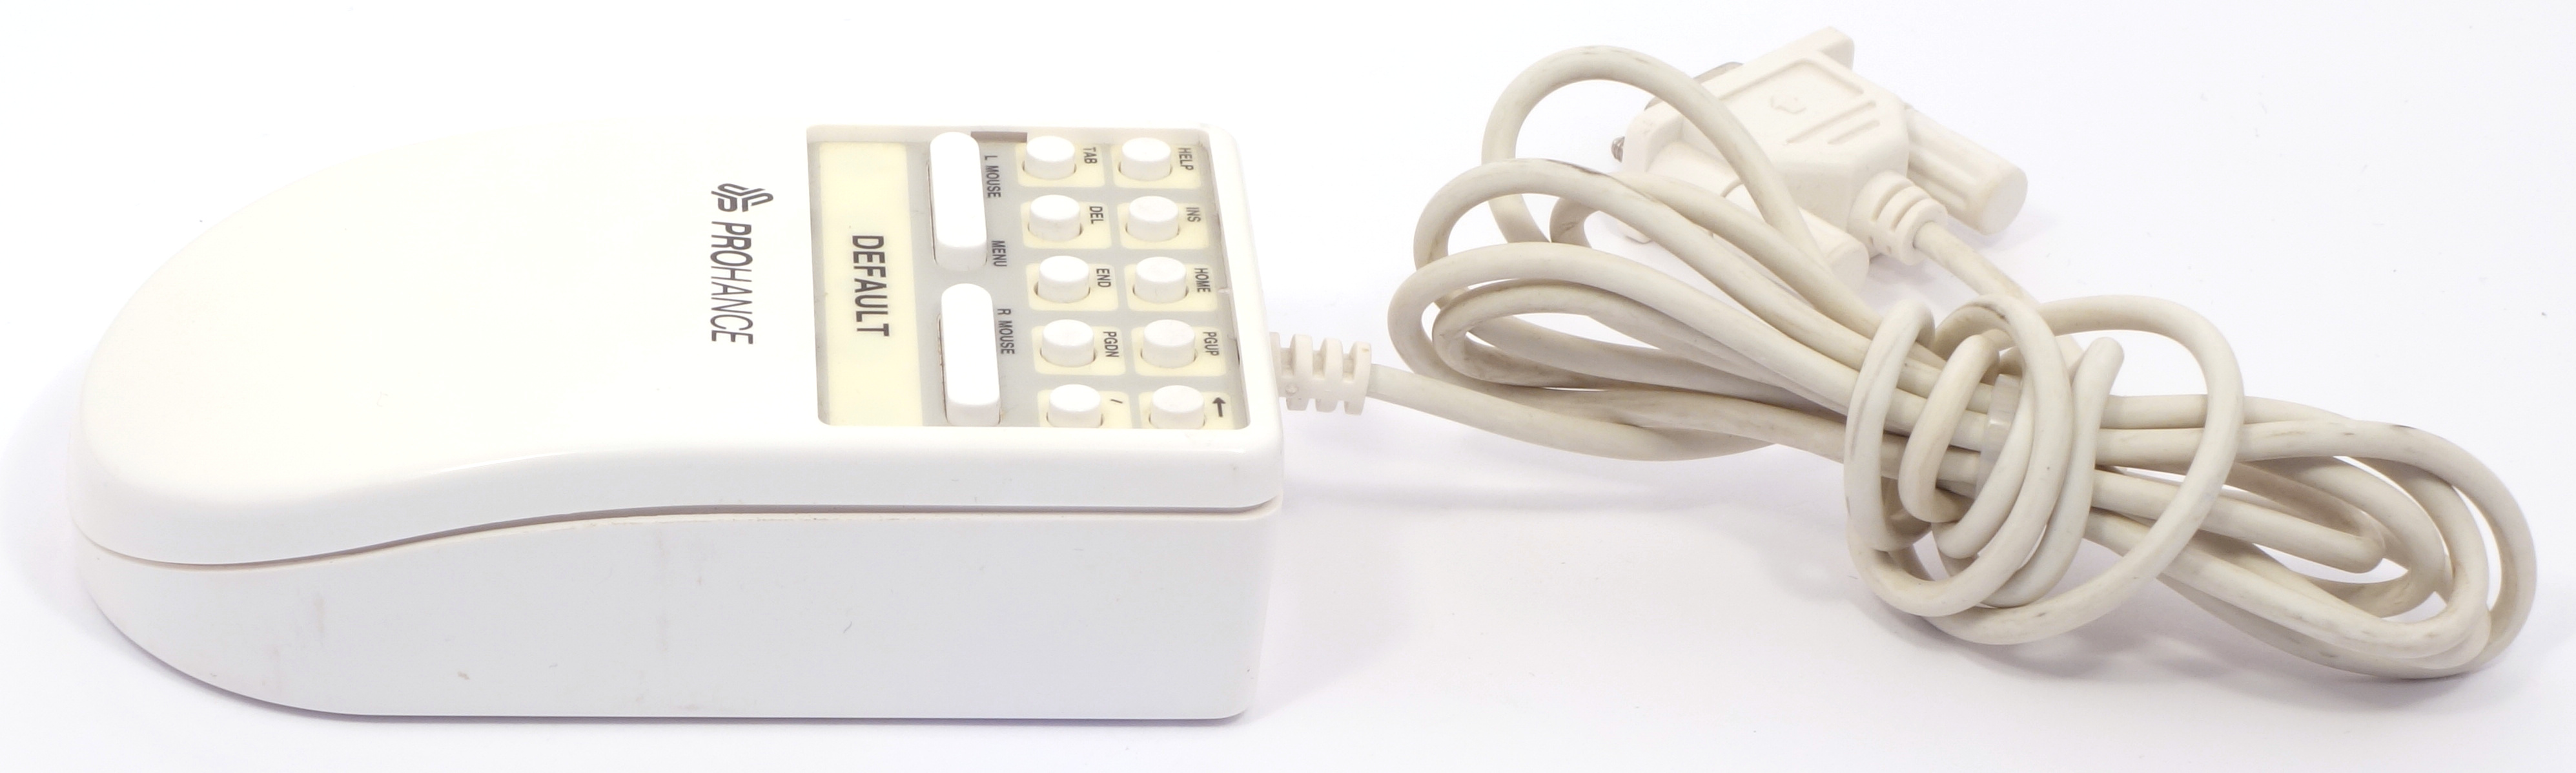
\includegraphics[scale=0.55]{1989_prohance_powermouse/pic_30.jpg}
    \caption{Изображение Prohance mouse}
    \label{fig:ProhancePhoto}
\end{figure}

Смысл использования данной мыши при работе с электронными таблицами Lotus 1-2-3 сводится к тому, что каждой функциональной клавише соответствует некая последовательность клавиатурных кодов, то есть фактически нажатие приводит к выполнению заданной макрокоманды. В остальном этот манипулятор действует как любая другая мышь, что позволяет использовать его с любыми графическими программами.

В плане эргономики корпус данного манипулятора повторяет форму мыши Microsoft, известной как <<Dove Bar mouse>>, в свою очередь позаимствовавшей форму у шлифовального бруска, и потому оказавшейся одной из первых эргономичных мышей (рис. \ref{fig:ProhanceSize}).

\begin{figure}[h]
    \centering
    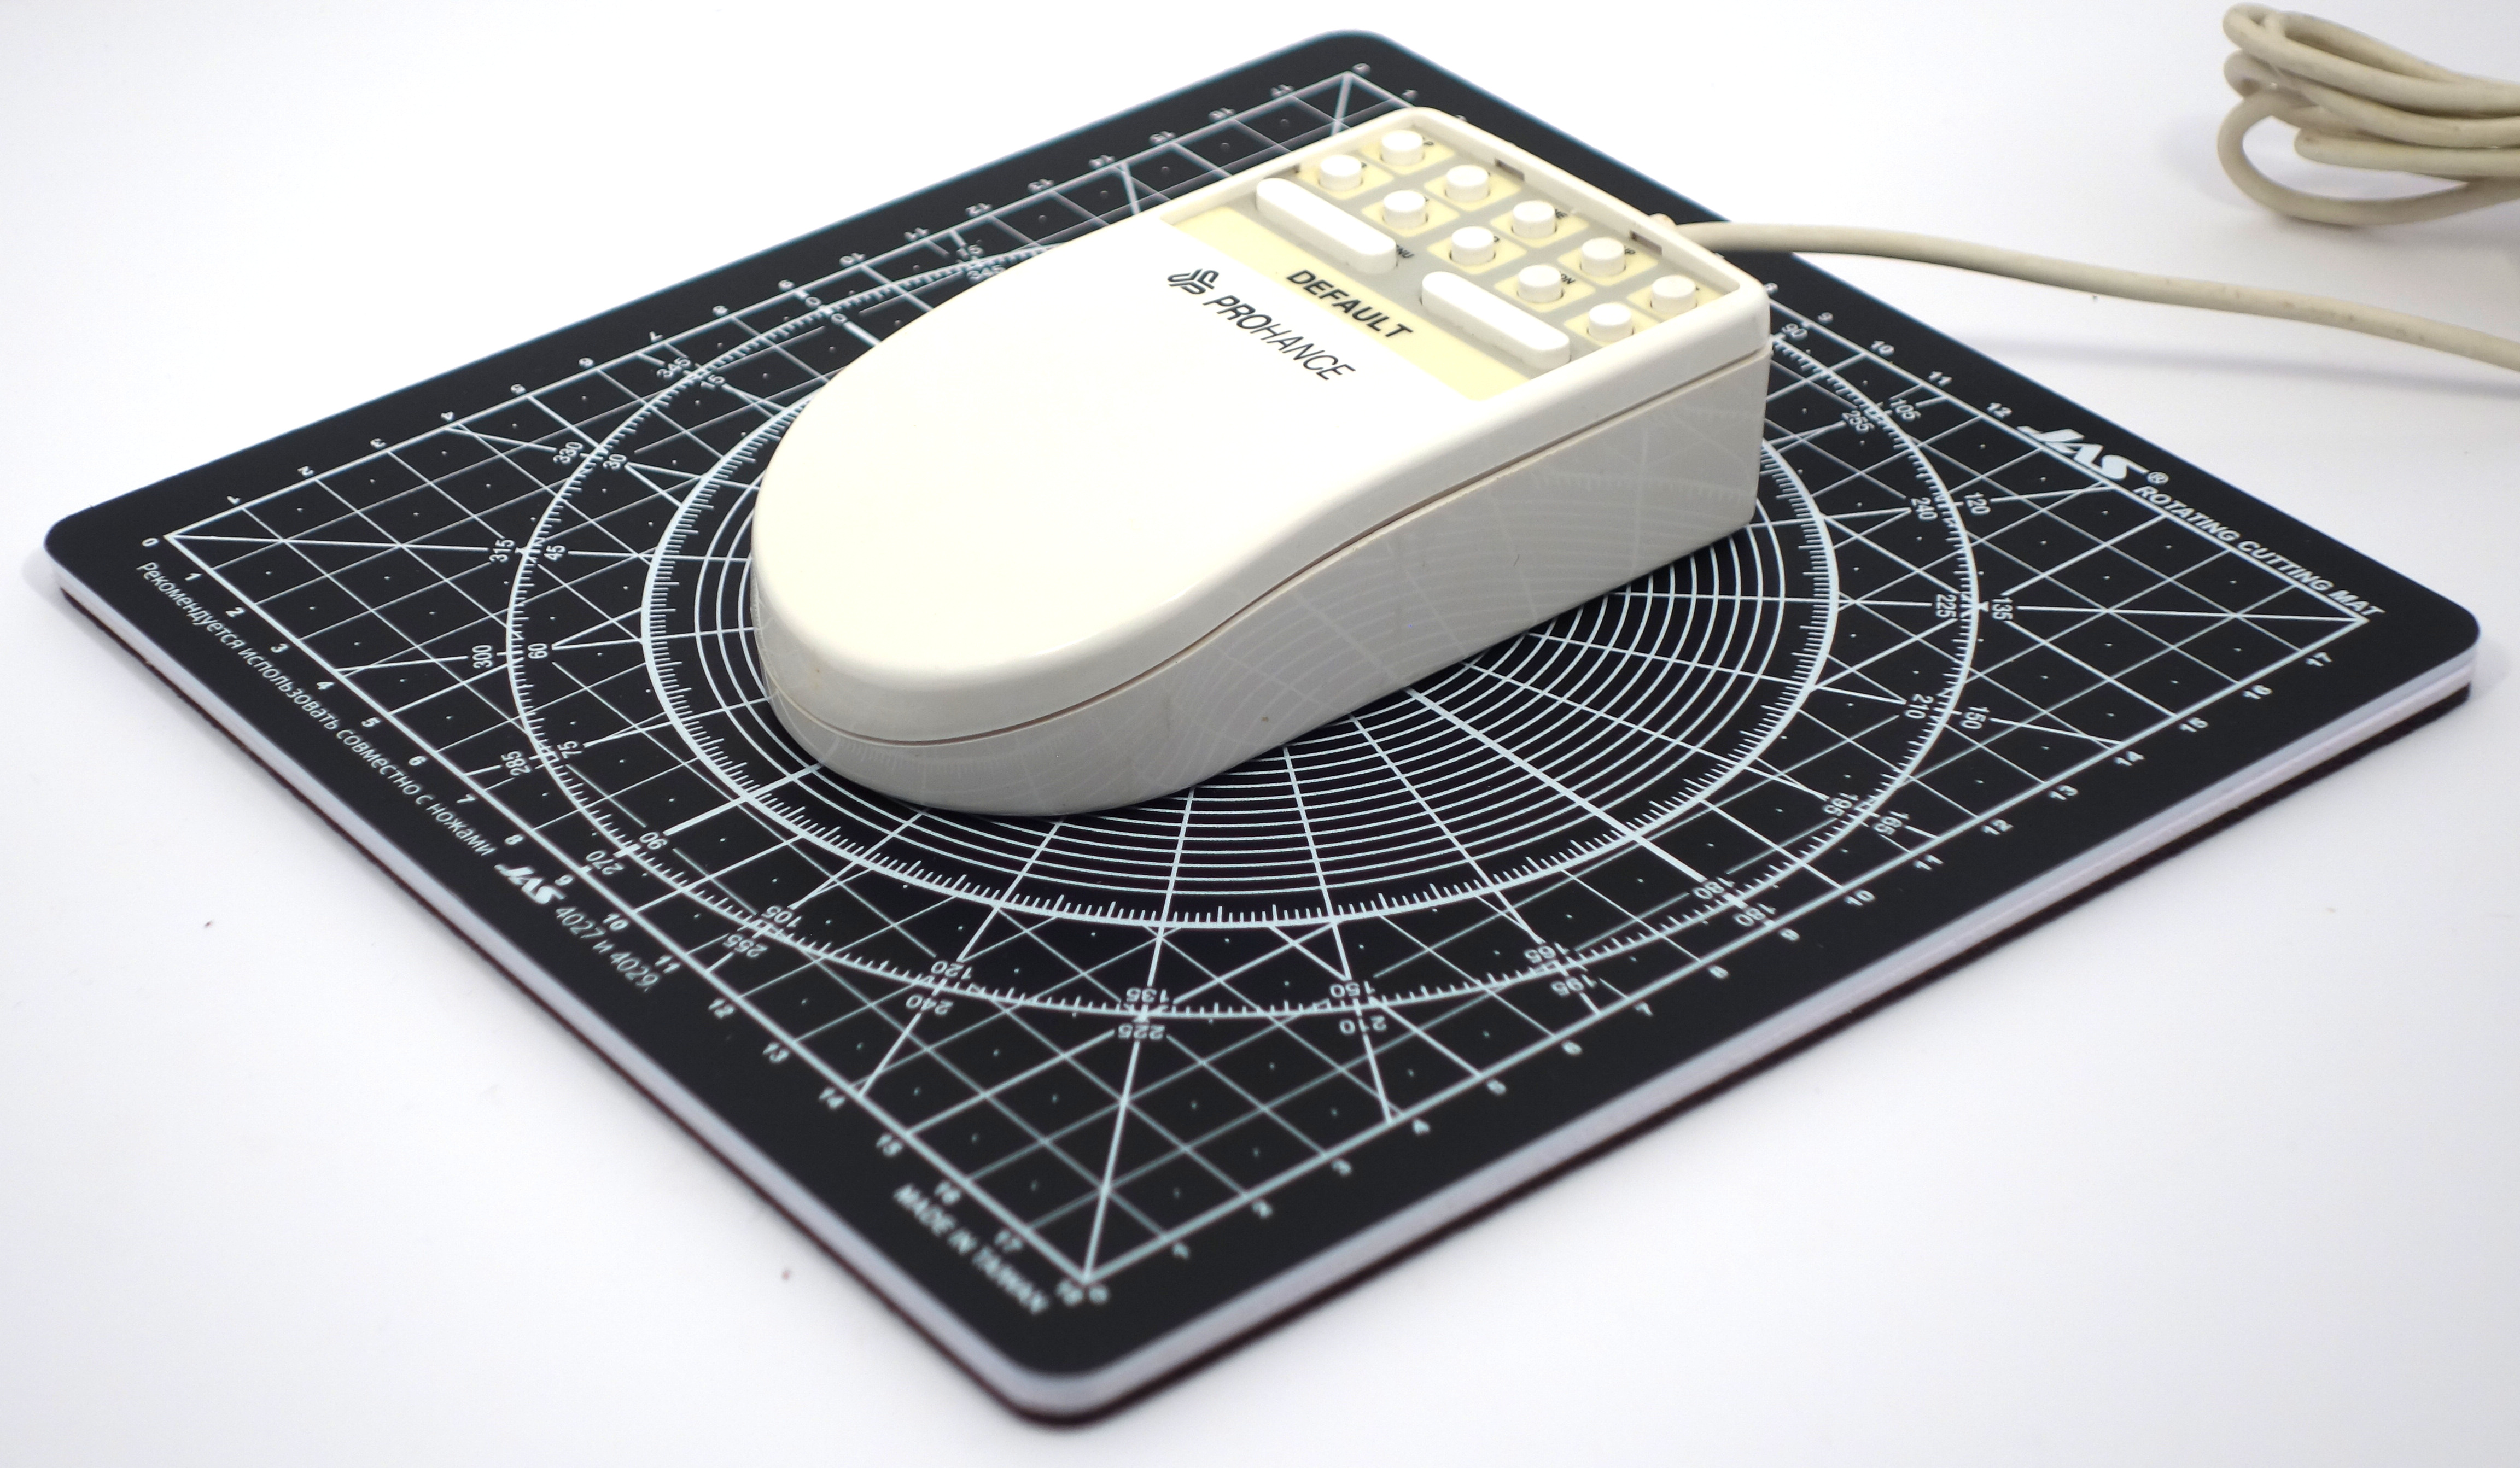
\includegraphics[scale=0.4]{1989_prohance_powermouse/size_30.jpg}
    \caption{Изображение Prohance Mouse на размерном коврике с шагом сетки 1~см}
    \label{fig:ProhanceSize}
\end{figure}

Поэтому с точки зрения формы к Prohance PoverMouse нет претензий по части эргономики (в отличие от её старшего собрата PowerMouse 100 с его сорока функциональными клавишами). Однако важным недостатком является размер клавиш: как основные кнопки, так и дополнительные клавиши Prohance имеют очень маленькую площадь, что весьма невыгодно отличает их от похожей по форме мыши Microsoft. Колпачки клавиш резиновые, как у микрокалькулятора, и издают едва слышный клик при нажатии. При этом они имеют некоторый запас хода, поэтому вероятность случайного срабатывания мала.

Сами по себе колпачки кнопок не содержат тактильных или визуальных отличительных признаков. Это особенно проблемно для функциональных клавиш: они имеют круглые колпачки одинакового размера, поэтому перед нажатием нужно внимательно следить за правильным положением пальцев. Для идентификации клавиш предусмотрены сменные вставки - накладки, размещаемые поверх функциональной клавиатуры. Однако из-за размера мыши эти надписи достаточно мелкие, перекрываются пальцами, и нетренированному пользователю приходится пристально их рассматривать, чтобы найти нужную (разница в размерах подушечки пальца и функциональной кнопки хорошо видна на рис. \ref{fig:ProhanceHand}).

\begin{figure}[h]
    \centering
    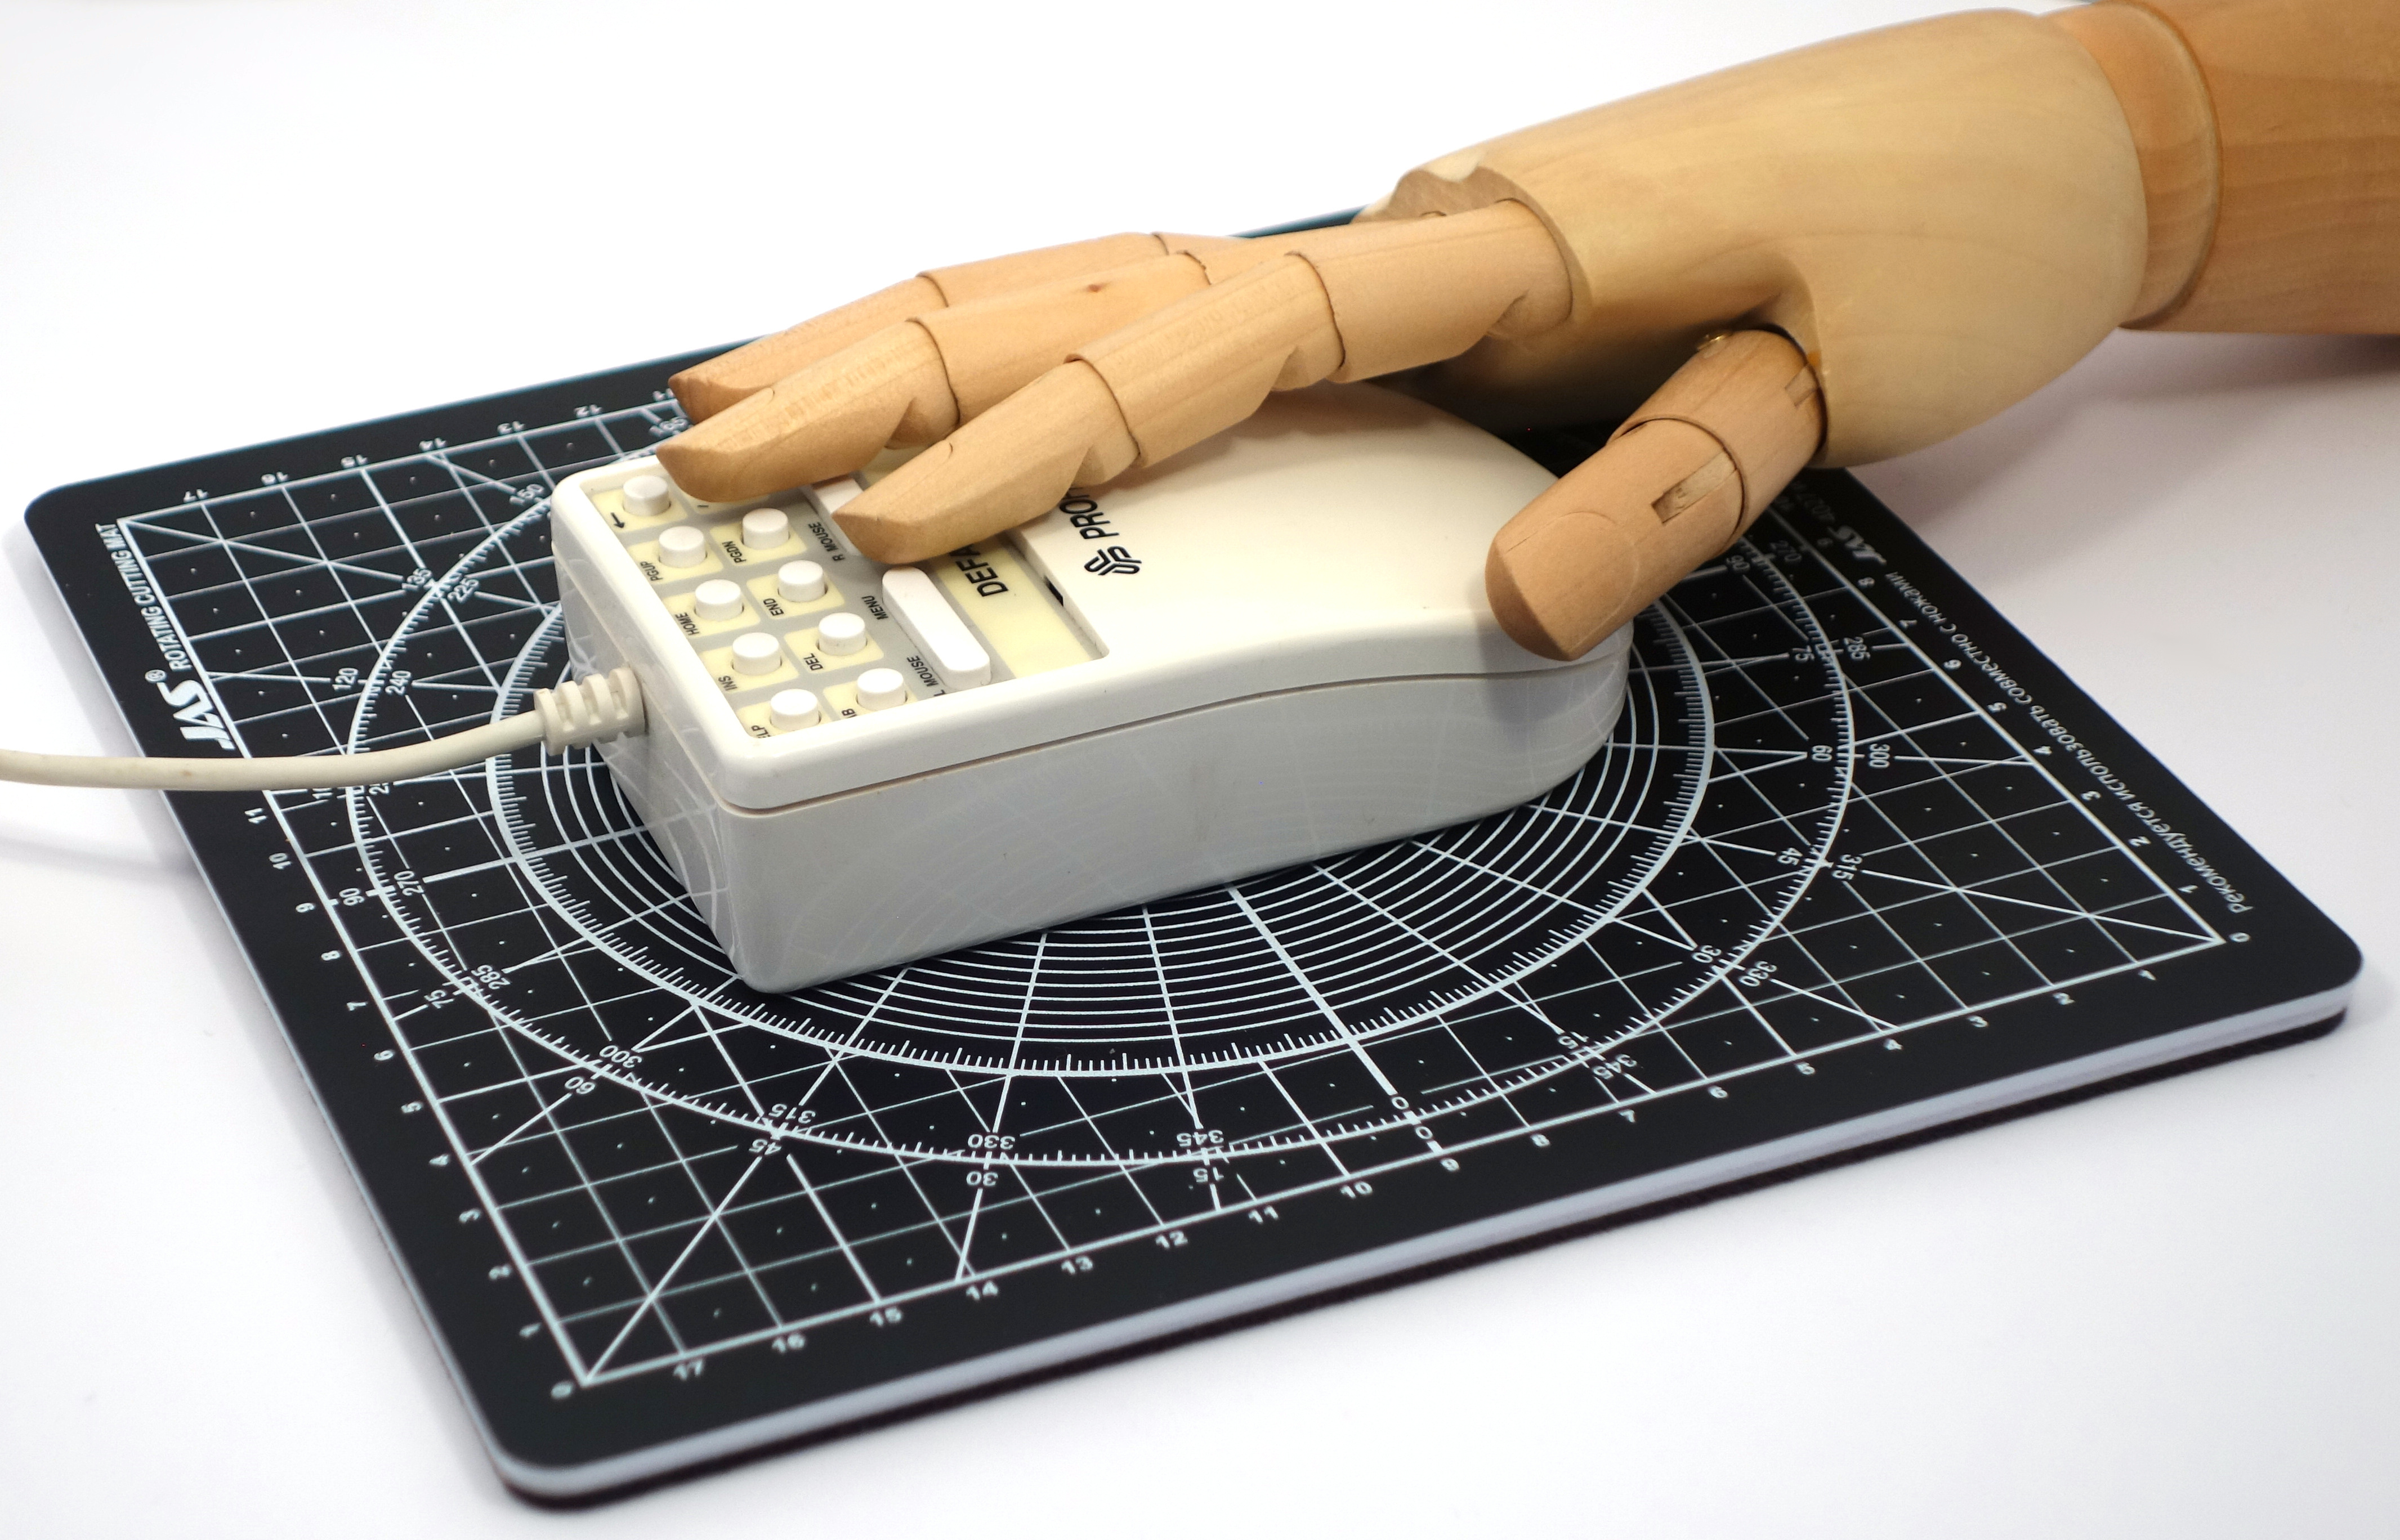
\includegraphics[scale=0.4]{1989_prohance_powermouse/hand_30.jpg}
    \caption{Изображение Prohance Mouse с моделью руки человека}
    \label{fig:ProhanceHand}
\end{figure}

Поэтому в целом Prohance PowerMouse получала негативные отзывы пользователей, вынужденных нажимать на чрезвычайно узкие левую и правую кнопки мыши, и вглядываться в мелкие надписи между рядами функциональных клавиш.

В \cite{prohance} отмечается, что в ранней версии драйвера содержались ошибки, приводившие к неадекватной работе мыши в Microsoft Word (даже ее незначительное перемещение приводило к пролистыванию страниц), исправленные в обновленной версии. Также отмечалась некоторая программная несовместимость с драйвером мыши Microsoft, приводившая к неработоспособности мыши в части приложений.

При этом настройка Prohance через комплектное программное обеспечение достаточно простая. В отличие от других мышей того времени, у Prohance нет программно реализованных экранных меню "--- вместо этого предлагается использовать переназначение функциональных клавиш. Prohance предоставляет функцию записи макросов, которая позволяет определять новые шаблоны для ее функциональных клавиш, а также изменять существующие.
Драйвер также позволяет задавать через конфигурационный файл уровень чувствительности мыши, однако функция динамического регулирования ускорения мыши предусмотрена не была.

\begin{figure}[h]
    \centering
    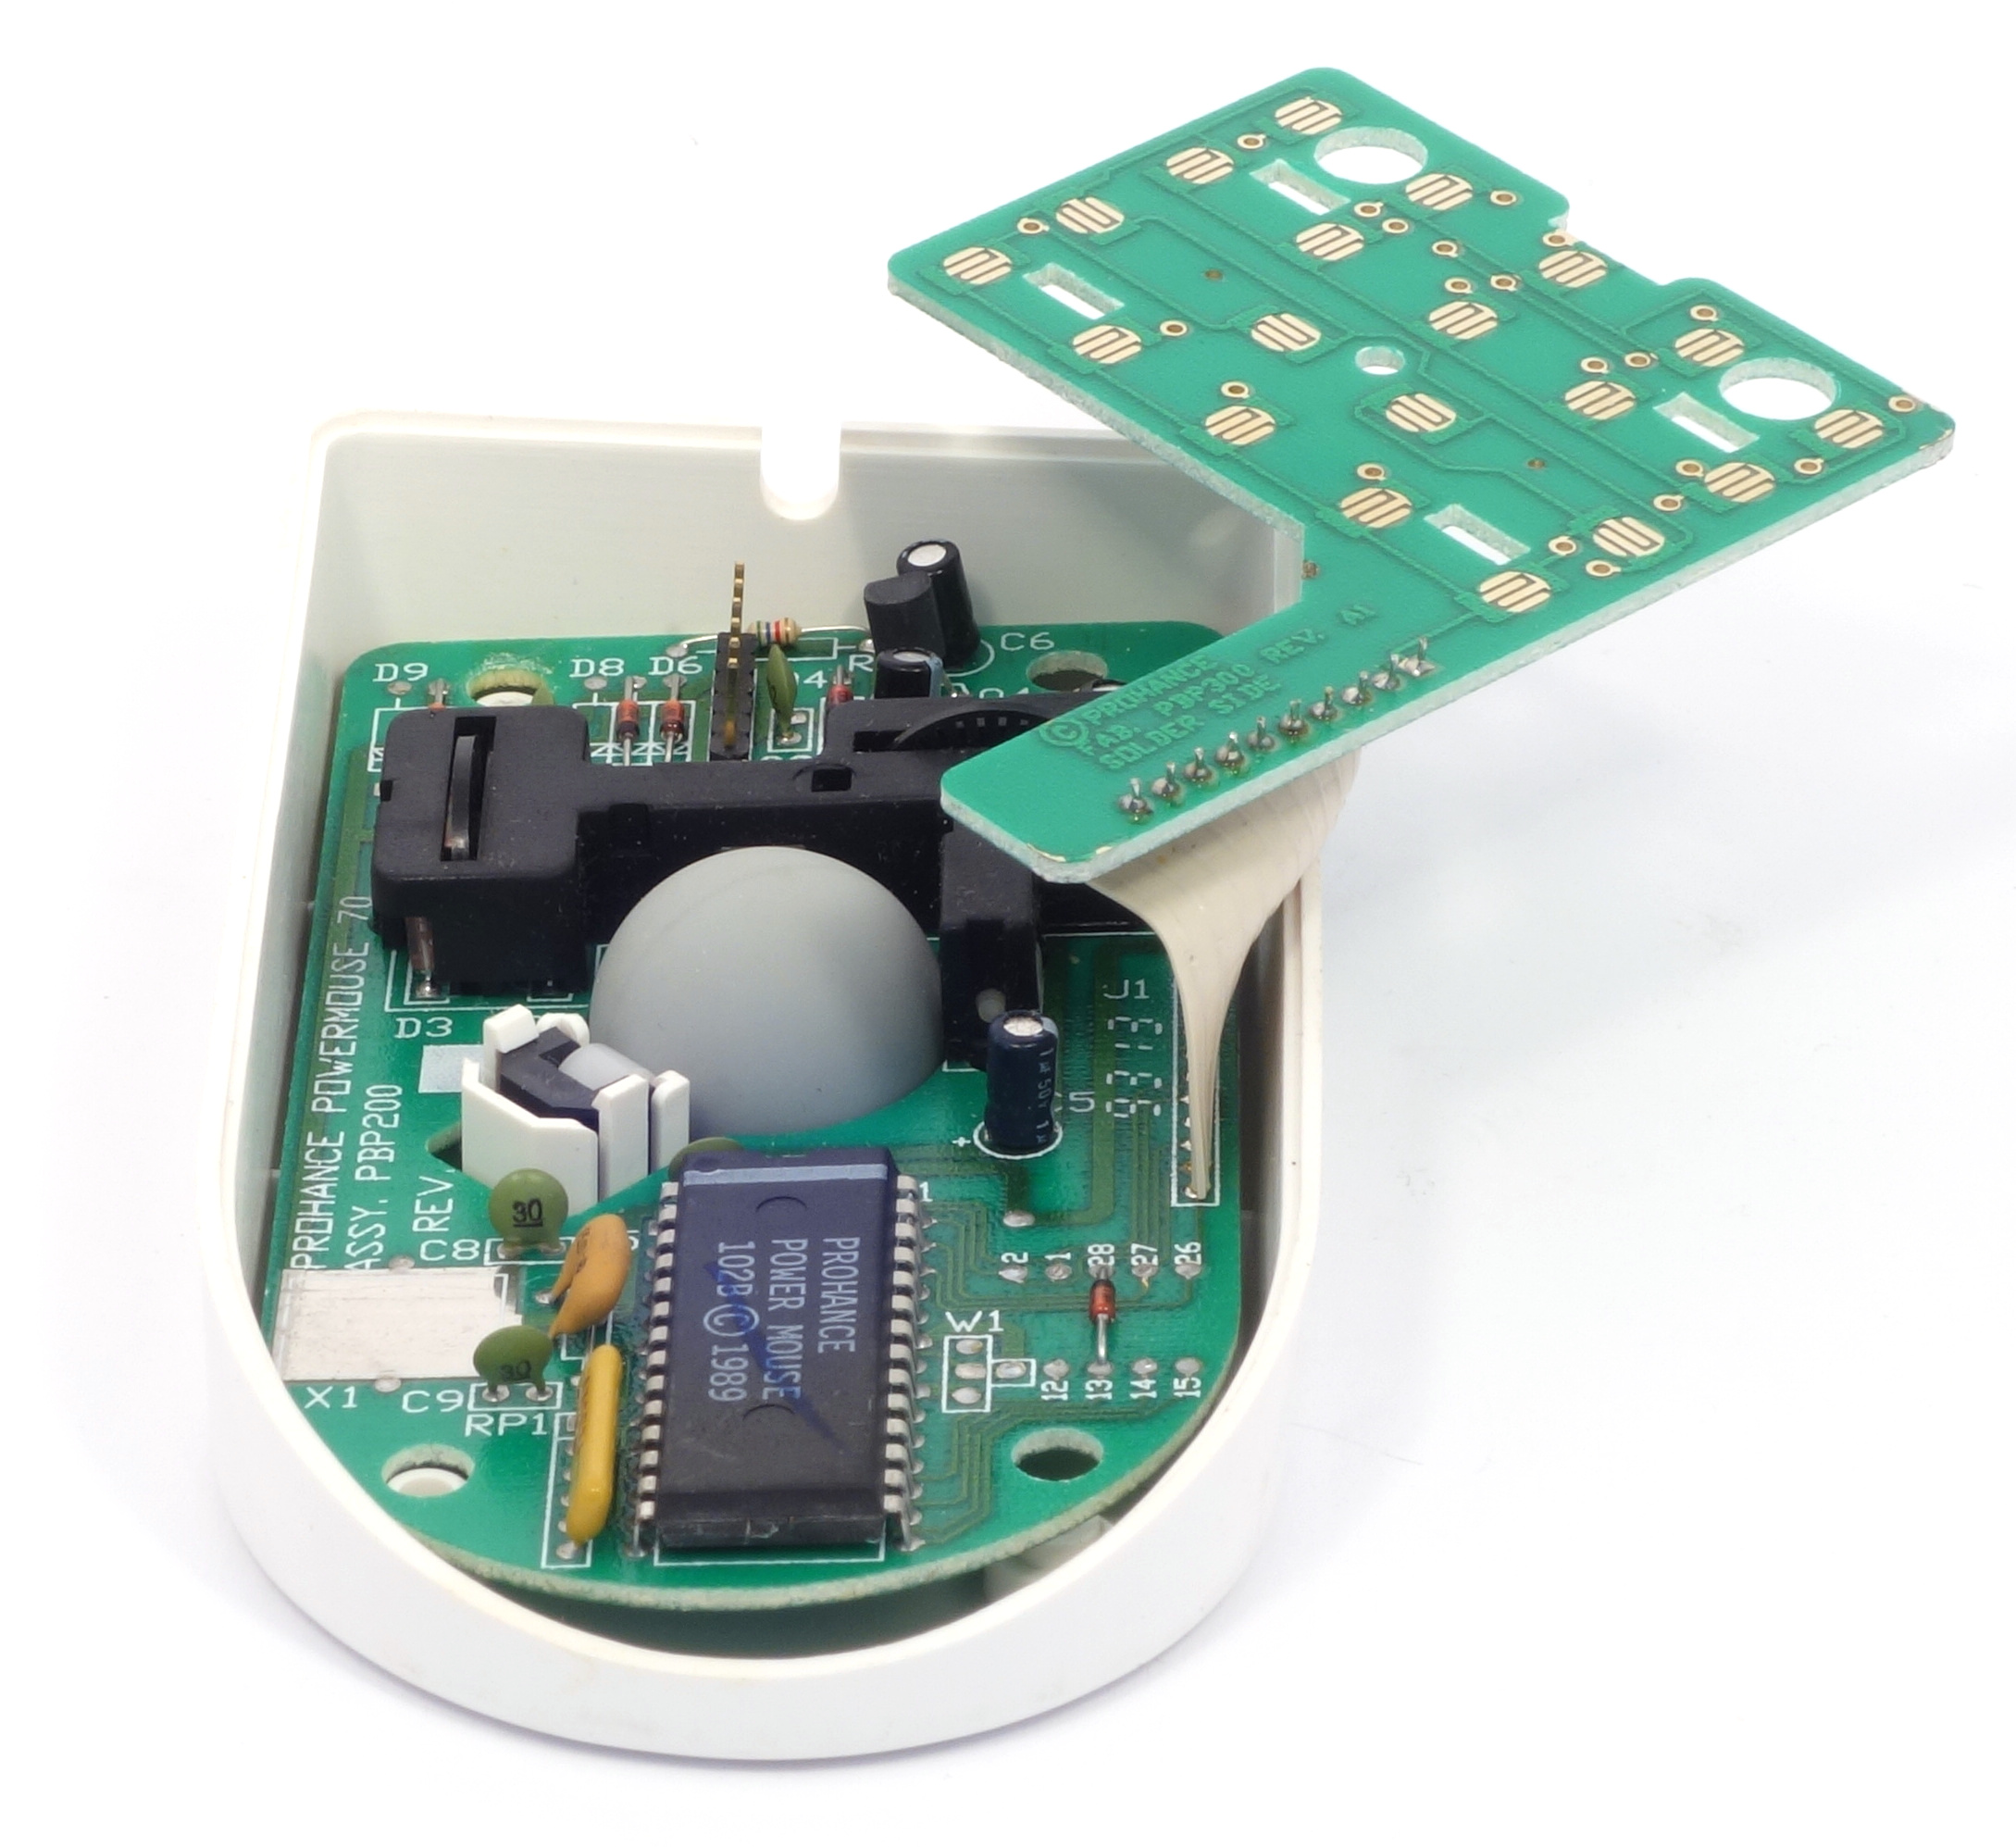
\includegraphics[scale=0.8]{1989_prohance_powermouse/inside_60.jpg}
    \caption{Изображение Prohance в разобранном виде}
    \label{fig:ProhanceInside}
\end{figure}

Мышь в разобранном виде показана на рис. \ref{fig:ProhanceInside}. Как можно видеть, она представляет собой типичную для начала 90-х годов оптомеханическую конструкцию, а блок кнопок и функциональных клавиш выполнен на отдельной печатной плате и является миниатюрной мембранной клавиатурой, аналогичной устанавливаемым в карманных микрокалькуляторах. Также на печатной плате можно разглядеть надпись <<PROHANCE POWERMOUSE 70>>, что отличается от номера, под которым модель поступила в продажу.

\begin{thebibliography}{9}
\bibitem{livingston} Livingston B. Genetically engineered mice run amok at Windows World // InfoWorld, Vol. 15, Iss. 21, May 24, 1989. - p. 34. \url{https://books.google.by/books?id=PTsEAAAAMBAJ&lpg=PA34&dq=prohance%20mouse&hl=ru&pg=PA34#v=onepage&q=prohance%20mouse&f=false}
\bibitem{prohance} Gruman G. What price mice? // Infoworld, V. 12, No. 17, April 23, 1990. - P. 63-69. \url{https://books.google.by/books?id=LTsEAAAAMBAJ&lpg=PA63&ots=GzwI8rKvl3&dq=%22prohance%20powermouse%22&pg=PA63#v=onepage&q&f=false}
\end{thebibliography}
\end{document}
